\documentclass[12pt, letterpaper]{article}
\usepackage{xcolor}  % For coloring text
\usepackage { bm , amssymb , amsthm }
\usepackage [ utf8 ]{ inputenc }
\usepackage[T1]{fontenc}
\usepackage{lmodern}
\newcommand*{\tab}{\texttt{\hspace*{1cm}}}
\newcommand*{\esc}[1]{\texttt{\textbackslash #1}}
\newcommand*{\gap}{\texttt{\hspace{2pt}}}

\usepackage{tikz}
\usetikzlibrary{automata,positioning}

\begin{document}

\section{Identifier}

\noindent
\textbf{IDENTIFIER\_OR\_KEYWORD}: \\
\tab \texttt{XID\_Start} \\
\tab \texttt{(XID\_Continue\gap{}|\gap{}\_XID\_Continue)\textsuperscript{*}}

\noindent
\textbf{RAW\_IDENTIFIER}: \\
\tab \texttt{r\#IDENTIFIER\_OR\_KEYWORD}

\noindent
\textbf{NON\_KEYWORD\_IDENTIFIER}: \\ 
\tab \texttt{IDENTIFIER\_OR\_KEYWORD\textsubscript{\textit{Except a \textcolor{cyan}{strict} or \textcolor{cyan}{reserved} keyword}}}

\noindent
\textbf{IDENTIFIER}: \\ 
\tab \texttt{NON\_KEYWORD\_IDENTIFIER\gap{}|\gap{}RAW\_IDENTIFIER}

\section{Comment}

\noindent
\textbf{LINE\_COMMENT}: \\ 
\tab \texttt{//(!!\gap{}|\gap{}@@\gap{}|\gap{}[$^\wedge$!@\esc{n}\esc{r}])[\bm{$^\wedge$}\esc{n}\esc{r}]\textsuperscript{*}}

\noindent
\textbf{INNER\_LINE\_DOC}: \\ 
\tab \texttt{//![\bm{$^\wedge$}!\esc{n}\esc{r}][\bm{$^\wedge$}\esc{n}\esc{r}]\textsuperscript{*}}

\noindent
\textbf{OUTER\_LINE\_DOC}: \\ 
\tab \texttt{//@[\bm{$^\wedge$}@\esc{n}\esc{r}][\bm{$^\wedge$}\esc{n}\esc{r}]\textsuperscript{*}}

\noindent
\textbf{BLOCK\_DOC\_OR\_COMMENT}: \\
\tab \texttt{BLOCK\_COMMENT} \\
\tab \texttt{| INNER\_BLOCK\_DOC} \\
\tab \texttt{| OUTER\_BLOCK\_DOC}

\noindent
\textbf{BLOCK\_COMMENT}: \\
\tab \texttt{/*(!!\gap{}|\gap{}@@\gap{}|\gap{}[\bm{$^\wedge$}!@\esc{r}]\gap{}|\gap{}BLOCK\_DOC\_OR\_COMMENT)([\bm{$^\wedge$}(*/)]\gap{}|\gap{}BLOCK\_DOC\_OR\_COMMENT)\textsuperscript{*}*/}

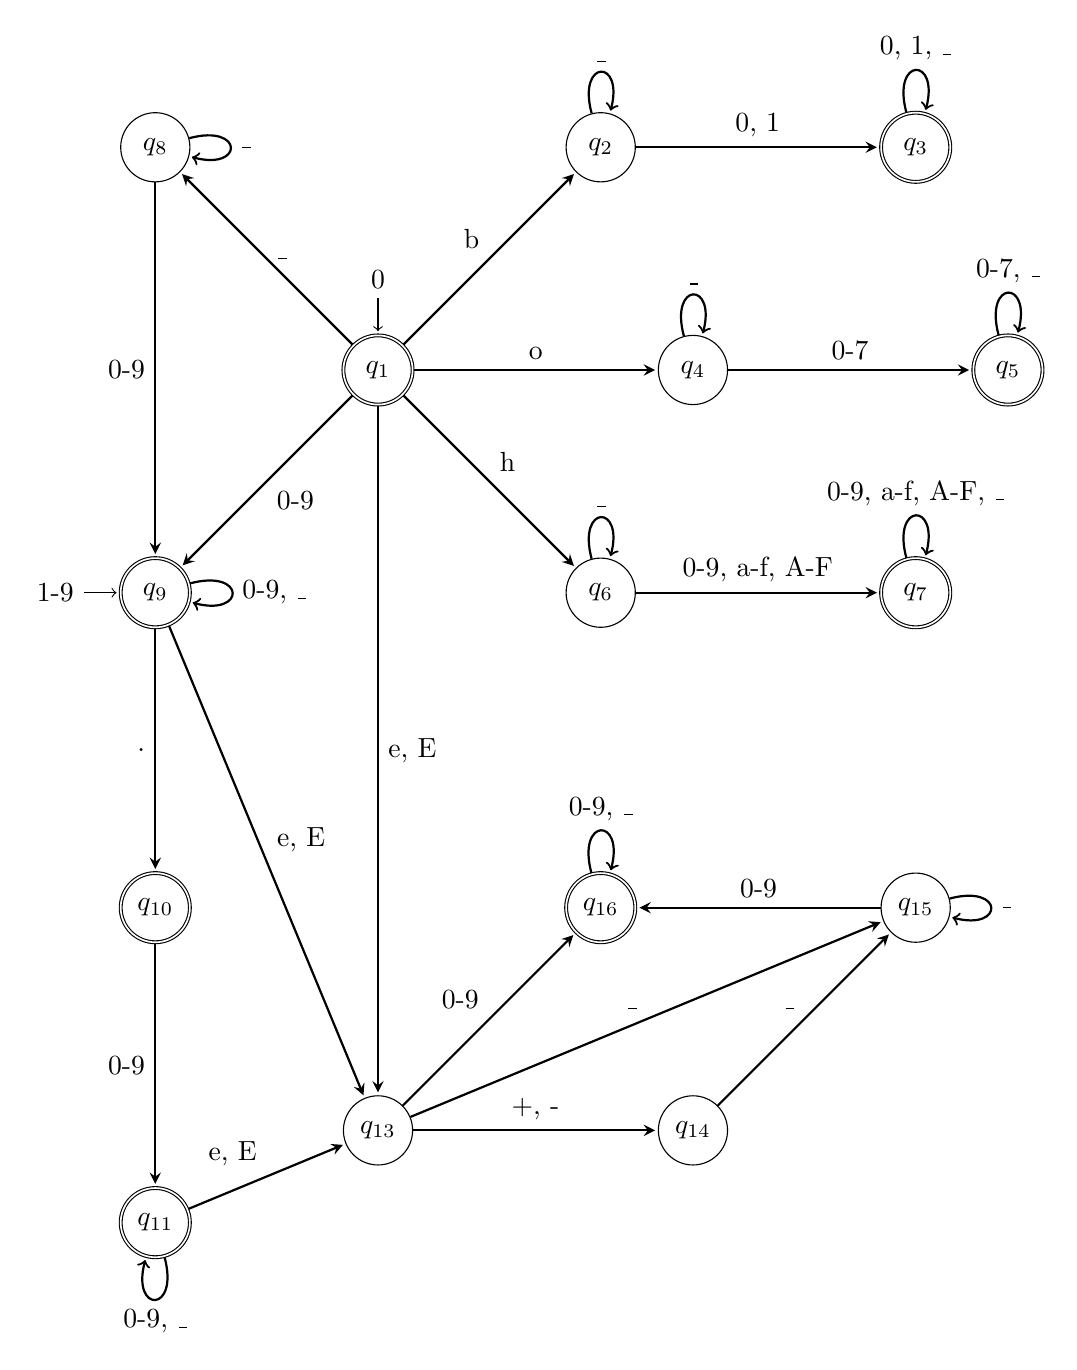
\begin{tikzpicture}[shorten >=1pt,node distance=4cm,on grid,auto] 
   \node[state,initial above, initial text = {0}, accepting] (q_1)   {$q_1$}; 
   \node[state] (q_2) [above right=of q_1] {$q_2$}; 
   \node[state,accepting] (q_3) [right=of q_2] {$q_3$}; 
   \node[state] (q_4) [right=of q_1] {$q_4$}; 
   \node[state,accepting] (q_5) [right=of q_4] {$q_5$}; 
   \node[state] (q_6) [below right=of q_1] {$q_6$}; 
   \node[state,accepting] (q_7) [right=of q_6] {$q_7$}; 
   \node[state,initial, initial text = {1-9}, accepting] (q_9) [below left=of q_1]   {$q_9$}; 
   \node[state] (q_8) [above left =of q_1] {$q_8$}; 
   \node[state, accepting] (q_16) [below =of q_6]   {$q_{16}$}; 
   \node[state] (q_13) [below left =of q_16] {$q_{13}$}; 
   \node[state, accepting] (q_10) [below=of q_9] {$q_{10}$}; 
   \node[state, accepting] (q_11) [below=of q_10]   {$q_{11}$}; 
   \node[state] (q_14) [right=of q_13] {$q_{14}$}; 
   \node[state] (q_15) [right =of q_16] {$q_{15}$}; 

    \path[-stealth, thick] 
    (q_1) edge node {b} (q_2)
          edge node {o} (q_4)
          edge node {h} (q_6)
          edge node [right] {\_} (q_8)
          edge node {0-9} (q_9)
          edge node {e, E} (q_13)
    (q_2) edge node {0, 1} (q_3) 
          edge [loop above] node {\_} ()
    (q_3) edge [loop above] node {0, 1, \_} ()
    (q_4) edge node {0-7} (q_5) 
          edge [loop above] node {\_} ()
    (q_5) edge [loop above] node {0-7, \_} ()
    (q_6) edge node {0-9, a-f, A-F} (q_7) 
          edge [loop above] node {\_} ()
    (q_7) edge [loop above] node {0-9, a-f, A-F, \_} ()
    (q_8) edge [loop right] node {\_} ()
          edge node [left] {0-9} (q_9)
    (q_9) edge [loop right] node {0-9, \_} ()
          edge node [left] {.} (q_10)
          edge node {e, E} (q_13)
    (q_10) edge node [left] {0-9} (q_11)
    (q_11) edge [loop below] node {0-9, \_} ()
           edge node {e, E} (q_13)
    (q_13) edge node {+, -} (q_14)
           edge node {\_} (q_15)
           edge node {0-9} (q_16)
    (q_14) edge node {\_} (q_15)
    (q_15) edge [loop right] node {\_} ()
           edge node [above] {0-9} (q_16)
    (q_16) edge [loop above] node {0-9, \_} ();
\end{tikzpicture}

% This line here is a comment. It will not be typeset in the document.
\end{document}
